%%
%% LaTeX Hetare Template
%%
%% Author: Yasunori Yusa
%%
%%%%%%%%%%%%%%%%%%%%%%%%%%%%%%%%%%%%%%%%
%
% # ビルド方法
%
%     % platex latex_hetare_template.tex
%
% DVI ファイルその他が出力される。
%
%     % dvipdfmx latex_hetare_template.dvi
%
% PDF ファイルが出力される。
%
% または、付属の Makefile を使って自動化する。
%
%     % make
%
% # トラブルシューティング
%
% ## PDF が文字化けする。
%
% latex_hetare_template.tex の文字コードに注意する。
% このテンプレートは Ubuntu 12.10 以降の platex のデフォルトの
% UTF-8 (改行コードは LF) を基本とする。
% とりあえず、ソースコードを変換してみる。
%
%     % nkf -wLu --overwrite latex_hetare_template.tex
%
% あとは、platex で明示的に文字コードを指定してみる (Ubuntu 以外の環境で有効)。
%
%     % platex -kanji=utf8 latex_hetare_template.tex
%
% Ubuntu 12.04 以前は UTF-8 が使えないので EUC-JP などに変換して使う。
%
% ## 参考文献、数式、表、図の参照が ?? になる。
%
% platex を何回か実行する。通常は 2 回で十分。
% 仕組みを知りたい人は出力された latex_hetare_template.aux を参照。
%
% ## platex がエラーで止まったときに Ctrl+c で抜けられない。
%
% X (ただの大文字の X) を入力してターーーンッ!
% または、Ctrl+d を押してみる。
%
%%%%%%%%%%%%%%%%%%%%%%%%%%%%%%%%%%%%%%%%
%
% # 本文を書く前に
%
% まずはドキュメントクラスを読み込む。
% jsarticle.cls が定番 (読み込むときに拡張子は書かない)。
% 学位論文では jsbook.cls もよく使われる。
% 読み込むときにオプションを指定できる。
% フォントサイズ 11pt、用紙サイズ a4j 辺りがよく使われる。
%
\documentclass[14pt,a4j]{jsarticle}
%
% 続いてパッケージ (スタイルファイル) を読み込む。
% amsmath.sty と amssymb.sty と graphicx.sty が定番で、
% 何も考えずにとりあえず読み込んでおくのが一般的。
%
\usepackage{amsmath}  % アメリカ数学会の数式拡張。
\usepackage{amssymb}  % アメリカ数学会の数学記号拡張。
\usepackage[dvipdfmx]{graphicx} % 画像関連のコマンドを提供する。
%
% 準定番なパッケージもいくつか紹介する。
%
\usepackage[margin=25truemm]{geometry} % 余白を設定する。上下左右 25 mm の例。
\usepackage{cite} % \cite{} の順番を自動調整してくれる。[3, 5, 4, 1] -> [1, 3-5]
\usepackage{url} % \url{} コマンドを有効にする。URL やメールアドレスに使う。
%
% 中級者以上が日常的に使っているパッケージもいくつか紹介する。
% これらのパッケージは、ただ読み込むだけじゃなくて、
% いくらか中級者的な設定をする必要がある。
%
% \usepackage{hyperref} % PDF にしおりを付ける。
% \usepackage{fancyhdr} % ヘッダ、フッタを調整する。
% \usepackage{algorithm,algorithmic} % 擬似コード
% \usepackage{listings} % ソースコード
%
% ついでに、かなりマニアックだけど欧文フォント関連パッケージも紹介してみる。
% デフォルトの欧文フォントはこれらとは違って
% Computer Modern という LaTeX 独自のもの。
%
\usepackage{txfonts}  % 本文セリフ体・数式に Times を使う。
% \usepackage{pxfonts}  % 本文セリフ体・数式に Palatino を使う。
% \usepackage{mathptmx} % 本文セリフ体・数式に Times を使う。txfonts.sty とは別の実装。
% \usepackage{mathpazo} % 本文セリフ体・数式に Palatino を使う。pxfonts.sty とは別の実装。
\usepackage{helvet}   % 本文サンセリフ体に Helvetica を使う。
% \usepackage{avant}    % 本文サンセリフ体に Avant Garde Gothic を使う。
\usepackage{courier}  %j 本文モノスペースに Courier を使う。
%
% パッケージを読み込んだら、とりあえずタイトル、オーサー、日付を書く。
% この記述は別に必須ではないけど、よく書かれる。
% \LaTeX のように \ で始まる文字列は LaTeX のコマンドで、
% \LaTeX は LaTeX のロゴっぽいものを出力する。
% その後ろの単独の \ はなんか空白をエスケープしている
% (これがないと LaTeX と Hetare がくっついてしまうため)。
% \thanks{}、\today も同様にコマンドで、
% 順に、オーサーの所属 (なくてもいい)、今日の日付を出力する。
%
\title{東京大学大学院工学系研究科システム創成学専攻 
\protect\\修士論文
\\広域での交通安全施策評価が可能な交通流シミュレータの開発
\\指導教員吉村忍教授}

\author{久保恒太\thanks{東京大学大学院工学系研究科システム創成学専攻}}
\date{\today}
%
% あとは、独自のコマンドを定義するときはこの辺に書く。
% \newcommand{コマンド}{定義} という書式で書く。
% ここでは、よく使われる \diff と \bvec{} を書いておく。
%
\newcommand{\diff}{\mathrm{d}} % 全微分の d はローマン体だよ派がよく使う。
\newcommand{\bvec}[1]{\mbox{\boldmath $#1$}} % 行列・ベクトルはボールドイタリック体だよ派がよく使う。
%
% さて、以上のようなヘッダ (プリアンブルと呼ぶ) を書き終わったら本文を始める。
% これ以降、\begin{} と \end{} というコマンドをよく使う。
%
\begin{document}
%
% まずは、タイトル、オーサー、日付を出力する。
% \maketitle というコマンドを書くと、
% ドキュメントクラス (jsarticle.cls) で定義されている見た目で出力される。
%
\maketitle
%
% タイトルの次には、アブストラクトを書く (省略可能)。
%
%
% いよいよ本文だが、まずは章立てのコマンドを紹介する。
% 順に、部、章、節、小節、小々節。
%
% * \part{}
% * \chapter{}
% * \section{}
% * \subsection{}
% * \subsubsection{}
%
% jsarticle.cls では \section{} から始めるのが一般的。
% jsbook.cls では \part{} や \chapter{} から始める。
%
\newpage

\tableofcontents
\newpage

\section{序論}

\subsection{研究の背景}
 国土交通省では平成27年までに24時間死者数を3,000人以下に、死傷者数を70万人以下とすることで、世界一安全な道路交通を実現するという目標を掲げている。また、死傷事故の約70%が道路全体の20%の区間に集中しているという事実から、幹線道路の中でも特に危険な箇所を特定し、その箇所に対して重点的に対策を仕掛けている。
道路改良による対策としては、右折レーンの延伸、歩道の整備、最高速度制限などが挙げられる。また、交通安全施設の設置としては、防護柵、導流表示、注意喚起表示(LED表示)などの設置が挙げられる。\\
 これらの道路や施設設置による従来までの対策に対して、近年の傾向としては交通事故対策として、高度交通システム(ITS)\cite{ITS-Japan}と呼ばれる,IT技術を駆使し、人と道路と自動車の間で情報の受発信を行い、道路交通が抱える事故や渋滞、環境対策など、様々な課題を解決するためのシステムを利用したものも登場している。交通安全支援のITSであるITSスポットサービス\cite{MLIT-1}では、道路に設置にされたITSスポットから車載されているカーナビに対して情報を送る。これにより、カーブなどの見通しが悪い場所でも近くに車がいることをITSスポットが知らせることで、事前に事故を防ぐことができる。他にも、車両前方のレーダーが先行車を察知し、追突の危険が高まった場合には自動的にブレーキをかけることで追突事故を未然に防ぐ、自動車被害軽減ブレーキ\cite{MLIT-2}などがある。\\
 このような国土交通省をはじめとした,行政の重点的な交通事故対策により,日本の事故死亡者は1992年から,また,事故発生件数は2004年から連続して減少傾向にある.図\ref{fig:accident-translation}に近年の交通事故による死者数および負傷者数を示す。しかし、依然として平成25年中の年間交通事故死者数は4,373人負傷者数は役78万人\cite{police2013}である.この数字が示すように交通事故は依然として大きな社会問題であり,交通事故をなくすことは国家の利益につながる.\\
\begin{figure}[ht]
  \centering
  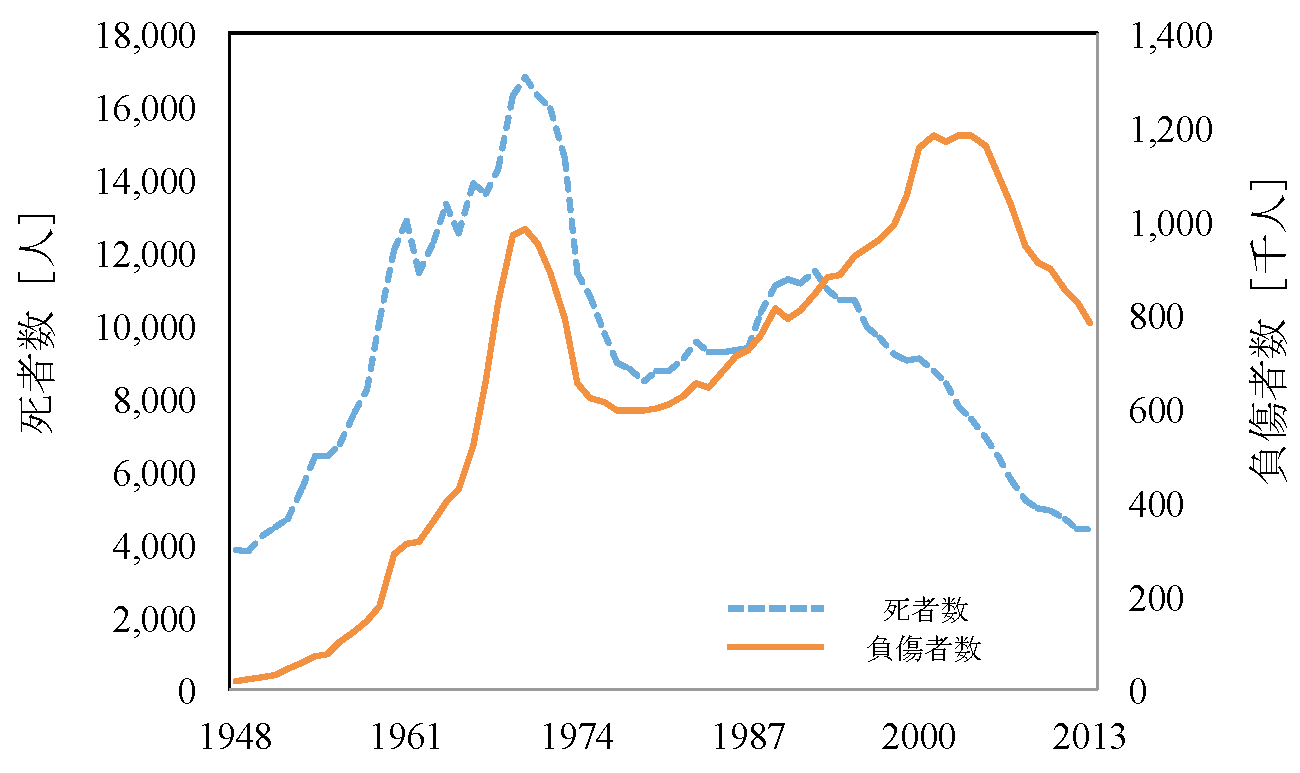
\includegraphics[width=1.0\hsize,bb=0 0 624 407]{./img/accident-translation.pdf} % 画像サイズ 320pt x 240pt の例
  \caption{交通事故死者数、負傷者数の推移}
  \label{fig:accident-translation}
\end{figure}
 この様な状況の中で交通事故に対して効果のある安全支援対策が待ち望まれるが、各対策を評価し、効率的に実施していくことが重要である。交通安全支援施策を評価しようとする時に、問題となるのが実験の困難さである。交通現象の実験では道路やその周辺施設を実験のたびに工事しては大きな費用がかかる。そのため、交通流シミュレーションによって、実際交通事故を再現できると,道路や交通規制の設計,ITS推進や交通教育への利用などによる事故状況の変化を仮想的に再現することでそれらの施策を評価することができる。こうした点で交通事故を再現する交通流シミュレータによる安全支援施策評価は事故の減少に寄与すると考えられる。
\subsection{交通事故シミュレーションの現状}
マルチエージェントを用いた交通流シミュレーションに関する研究は現在まで、多くされてきた。それらの研究は交通渋滞に関するものなどが多く、交通事故に関するものは少ない。その理由としては、そもそも交通事故をモデル化することが難しいことなどが挙げられる。こういった中で行われてきた既存研究では交様々なモデルを提案し交通事故の再現してきた。
田中らの研究では認知エラー・判断エラー
自動車の運転行動は認知・判断・操作の3つの過程に分類される.この3つの過程のどこかにエラー状態が起きた時に交通事故は発生する(2).既存の交通流シミュレータにおける交通事故の実装においても,この考え方に沿ったものが多い.認知段階におけるエラーでは,認知フィルタという概念により,ドライバ間での認知レベルの差を表した田中ら(3)のモデルや,藤井ら(4)の中心視野と周辺視野を考慮したモデルなどがある.また,古川ら(5)の研究はエージェントの判断によるエラーに踏み込んだものである.これらの研究では交通事故を実現象に近い形で再現してはいるものの,例えば,特定の交差点など局所での安全施策評価での利用に限られており,広域なシミュレーションには利用できず,実際に街路を設計する際の交通安全施策評価の実用性の問題が残る.このような現状から広域で利用できる交通流シミュレータが必要とされている.
\subsection{研究の目的}
本研究の目的は都市単位での様々な広域での交通安全施策評価が可能な交通流シミュレータの開発である.交通情報である道路形状、交通量、信号の配置、点灯、建物の情報を入力することで、事故情報である事故発生件数、事故形態、事故発生箇所などを出力するマルチエージェントシミュレーションである。具体的な利用方法としては、都市などで道路構造を変えたり、交通量が変化した時にどの様に事故が増えるか減るかなどを行政や地方自治体が試算するために利用するなどが考えられる。
\newpage
\section{研究手法}
\subsection{研究手法の特徴}
以下に本研究手法におけるにおける特徴を述べる。\\\\
\textbf{特徴1.複数のモデルに対する複数の事故をモデル化・実装}\\
 本研究においては、5つの事故である追突事故・出会い頭事故・右左折事故・車線変更・正面衝突事故を扱う。これらの事故が起こる過程においては、それぞれ別々のエラーが起こり、事故に繋がるというモデルになっている。交通事故をモデル化する際に汎用的な単一のモデルを用い様々な事故を再現するという手法もあるが、本研究では実際に起こりやすい事故について、事故が発生するまでのプロセスはそれぞれに違った現象であるという立場からこの手法を採用した。\\\\
\textbf{特徴2.認知・判断エラーをモデルに加味}\\
 認知・判断エラーについて説明する前に、自動車の運転行動について説明する。運転行動は一般的に認知・判断・操作の3つの過程に分類される\cite{ITARDA2005}。認知過程では、安全に通行するために必要な物を見る(発見する)ことであるが、これは単に見る
判断過程では、認知した対象がどのような行動をするのか、自分はどのように行動すればよいのか
操作過程では、判断や決定に従ってハンドルやブレーキなどを操作する。例えば赤信号における停止という運転行動では、赤信号を見て(認知),減速しようと考え(判断),ブレーキを踏む(操作)といった流れとなる.\\
 過去の研究においては認知エラーが採用されているものが多い、認知エラーによる事故は件数も多く、見えているかどうかということが物理的に比較的明確な現象なのでモデル化しやすいからである。これに対して判断エラーを考慮することは人間の思考の一部をモデル化することとなり、様々な考慮をしなければならない。古川らは交通事故シミュレーションを行う上でこの判断エラーを取り入れた\cite{Furukawa2009}。この研究ではUDM(Universal Design Model)というモデルを提案している。UDMにおける認知過程ではエージェントがそれぞれ現実の世界とは違う外部世界というものを保持している。エージェントは認知段階において外部世界に情報を蓄える、そして判断段階では現実の外部環境ではなく、外部世界から情報を参照する。また、ドライバは個性や心理状態に応じて運転欲求を持っており、の欲求に応じて判断を変えてリスク判断を行っていく。このリスク判断の部分については確率的な計算を行っている。外部世界モデルの概念はエージェントによって見えているものがそもそも違い、判断についてもその時々によって異なるということを表している点で現実の運転行動をよく表現していると考えられる。そのため、本研究ではモデルを構築する上で外部世界の概念を取り入れ、判断・認知エラーを加味することとする。操作段階におけるエラーについて事故件数が少ないとされているため,本研究では扱わない.\\\\
\textbf{特徴3.計算時間を考慮した簡易なモデル}\\
 本研究の目的とする広域での交通流シミュレーションを実現するためには計算時間の短縮が不可欠であるが、認知・判断過程でエージェントにエラーを起こすということは複雑な計算を行う場合が多く、計算量が多くなりがちである。藤井らの研究\cite{Fujii2011}は認知エラーに絞り単一のモデルから構築されており、ドライバに見えている景色を二次元の画像として、各ドライバのエージェントが持つことで、他のエージェントを認知できなくなった時に衝突の可能性がある。認知できるかどうかの判断については、中心視野、周辺視野を考慮している。この研究は人間の視覚を精緻に再現し、現実と近いものになってはいるものの、二次元の図を各タイムステップで描く必要があり、計算量が膨大となるため、広域での交通流シミュレーションには向かない。本研究では目的に合わせ、現実の事故を再現しながらも、簡易なモデルを構築するという手法で広域での交通流シミュレーションを実現する。

\newpage

\subsection{交通流シミュレータMATES}著者らが開発中の知的マルチエージェント交通流シミュレータMATES (Multi-Agent-base Traffic and EnvironmentSimulator)(6)に新たな認知・判断モデルを追加・実装する.MATESにおいてドライバはエージェントとしてモデル化されており,周囲の環境から情報を取得して自律的に行動する.また,複雑な交通流を再現可能であり.現実の現象に即した交通事故を再現するという本研究の目的に適した交通流シミュレータであるといえる.
\newpage
\subsection{交通事故の分類}
交通事故は分類して考えられる。図\ref{fig:accident-classification}は平成15年から平成25年までに起きた交通事故を分類分けをした円グラフである。このグラフは警察庁のデータ\cite{police2013}を元に作成した。
\begin{figure}[ht]
  \centering
  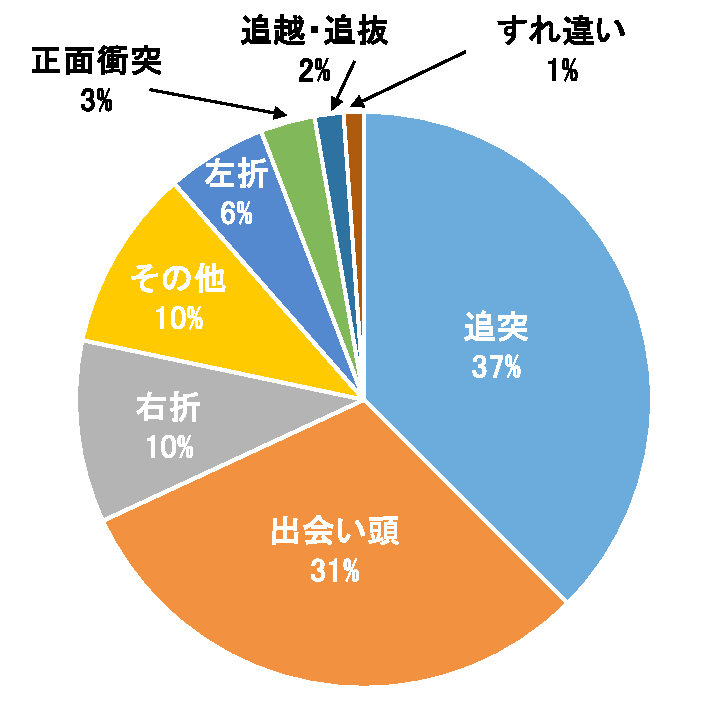
\includegraphics[width=0.5\hsize,bb=0 0 350 340]{./img/accident-classification.pdf} % 画像サイズ 320pt x 240pt の例
  \caption{平成15~25年における交通事故の分類}
  \label{fig:accident-classification}
\end{figure}

これによるとこの年に最も多かった事故は追突、ついで出会い頭事故、右折と続いている。その他が10%と少なく、事故の大部分が大まかに分類されているのがわかる。この様に現実の事故が分類できることから、本研究においても、これらの事故から代表的なものを取り出し、それぞれ個別にモデル化することで,より実現象に近い形で交通事故が発生することを目指す.これらの事故のモデル化に際しては自動車技術会が発表している交通事故予測シミュレーションシステム検証マニュアル\cite{manual2013}を参考にした.このマニュアルは予防安全策の開発において、その効果を予測・
故予測シミュレーションシステムが備えている機能レベルや交通状況の再現能力を評価するための標準的な検証・評価手続きを示したものである。以下に5つの事故の状況を述べる.\\\\
\textbf{(1) 追突}\\交差点手前で停止した先行車に追突.先行車は早い段階で停止したが,自車は先行車以外の対象物を認知していたもしくは,脇見しており,先行車を認知できないため追突する.\\\\
\textbf{(2) 出会い頭}\\ 交差点を直進で進入しようとした時,側方から他車が出てきたため,出会い頭の衝突.建物が密集していたため,他車の発見が遅れたと考えられる.\\\\
\textbf{(3) 右左折}\\ 交差点内で自車が右折しようとしているときに,対向車は左折もしくは直進をしようとし,自車の方が先に通過できると見誤ったために衝突\\\\
\textbf{(4) 進路変更}\\進路変更時,隣のレーン後方から車両が接近していることに気づかず進路変更を行ったため衝突\\\\
\textbf{(5) 正面衝突}\\ 脇見運転をしており,対向車線に進入したため衝突
\newpage
\subsection{エラーの分類}
また,交通事故の要因の分析を行った.この分類には自動車技術会の公開しているヒヤリハットデータや,山田らの交通事故シナリオの研究(8)を参考にした.その結果,事故要因を以下の3つに絞った.見えないことによる認知エラー,見ていないことによる認知エラー,傲慢な判断エラーである.これら4つのエラーについて説明する.\\\\
\textbf{(1)見えないことによる認知エラー}\\
 衝突しうる,また,その原因となりうる対象物(先行車,信号,並走車など,以降認知対象物とする)が物理的に見えない状態である.例えば見通しの悪い交差点などで側方から進入した車両と衝突する場合などはこの原因が強いと考えられる.\\\\
\textbf{(2)見ないことによる認知エラー}\\
 見ないことによる認知エラー: 物理的に認知対象物が見える状態であっても,ドライバが見ていないという状態と定義する.例えば脇見運転が該当する.\\\\
\textbf{(3)傲慢な判断エラー}\\
 認知対象物を認知している場合において,判断の誤りによって起こるエラーである.右折対左折の事故において,対向車を認知しつつも,対向車が道を譲ってくれると判断した時などはこのエラーを原因とする.また,見通しの悪い交差点で,左右確認をせずに交差点に進入する場合もこのエラーが原因の一つとなる.\\
これら4つのエラーを各事故に関して,実装した.
\newpage
\section{交通事故のモデル化}
\subsection{追突事故}
 追突事故は先行車の後方と、後方車の前方が追突することや、低速での発生が多いことから幸い死亡事故の割合は他の事故と比べて少ないものの、全体の事故の中でも37\%を締め絶対数としては最も多い事故である。交通事故研究センターの報告\cite{ITARDA2003}によると追突事故の原因の70%は多くは先行車以外のものを認知することや,脇見運転などである.(9) そのため,各タイムステップにおいて先行車以外の認知対象物が多いほど認知エラーが発生する確率が高くなるよう設定した.認知エラーが発生した時,自車は先行車を認知できなくなる.認知エラーが起きた後には,最後に先行車を認知した時に得られた先行車の速度情報をもとにその位置を外挿予測する.この様にして計算された先行車と自車の位置に乖離がある場合が置き換えによる判断エラーとなる.判断エラーが起きたために先行車の正確な位置を把握できず,追突事故が発生する可能性がある.
\subsection{出会い頭事故}
 出会い頭事故の多くは信号のない見通しの悪い交差点で発生している.そのため,本モデルでは信号のない交差点で建物等の遮蔽物があることで,遮蔽物に隠れた車両を認知できなくなるという,見えないことによる認知エラーを再現する.あわせて,見通し計算を行うことで視野の制限を判断した.見通し計算には二つの車両を結ぶ線分と遮蔽物である壁面との交点が存在するか判定するアルゴリズムを採用している(10).シミュレーション開始時に,遮蔽物がある交差点に繋がっている車線に対し,見通しが悪いという属性を付与することで,交差点に進入する全ての車両に見えないことによる認知エラーが発生する.この時,傲慢な判断エラーが起きていない車両は「遮蔽物の陰から車両が飛び出してくるかもしれない」と判断して一時停止するようにした.逆に判断エラーが起きている時,つまりは交錯する車両を予測しない時には一時停止せず,遮蔽物の陰から車両が進入してくるときに,事故が起きる可能性がある.
\subsection{右左折事故}
右左折事故は信号のある交差点で自車が左折しようとしてかつ対向車が右折をしようとしてきた時に発生するものである.交差点が前方に存在し,対向車が存在する場合に傲慢な判断エラーが起きる可能性がある.エラーが生じている場合には自車と対向車が交差点を通過し切る時間を計算して,自車の方が対向車より早く通過できると予測したとき,実際には交差点に進入すると衝突する可能性がある場合でも,交差点へ進入する.実際には対向車が先に交差点に進入すべき時に自車も交差点に進入することがあるため,衝突事故が起こる可能性がある.
\subsection{車線変更事故}
進路変更の事故は単路で発生する.進路変更を車両が行うときに,移動するレーンの前方及び後方を確認するが,見ないことによる認知エラーが起きた場合は後方に車両があった場合でも認知しない.また,このエラーが起きる確率計算に関しては追突事故と同じように,認知対象物が多ければ多いほど,エラーが生じる確率が高くなる.このため,進路変更先の後方車両と衝突する可能性がある.
\subsection{正面衝突事故}
正面衝突の事故では脇見や前方の不注意によって車両が対向車線に進入することが多い(11).そこで,対向車線に接する最内車線を走行中に認知対象物の有無に対して確率的にエラーを発生させる.この事故においても,追突,進路変更の事故と同様に認知対象物が多いほどエラー発生率が高くなっている.エラー発生時に,車両を対向車線側に移動するということとした.対向車両が存在するときに正面衝突の事故が起こる可能性がある.
\section{はじめに}
本文はただのふつうの文章なのでとにかくふつうに入力する。
ソースファイルの中で改行する場所は基本的に自由で、
改行が本文に反映されることはない。
MS Word だと好きなところで改行できるけど、
ふつうの文章で段落の途中で改行する必要とかないよねというのが \LaTeX 的思考。
改段落には空白行を一行入れる。
以降はよく使うコマンドを書いていく。
内容は LaTeX コマンドシート一覧\cite{list_commands}を参考にした。
このサイトは非常に便利なので何度も参照するといいと思う。
ちなみに、参考文献の参照には相互参照という仕組みを使う。
\LaTeX ではラベルを適当に付けて相互に参照することで、
参考文献、数式、図、表の番号がズレることを防止できる。
もちろん参考文献の参照を [1] のように直打ちするのもダメではない。
%
\section{空白と強制改行}
段落の中での改行は基本的にはやらないが、
強制改 \\ 行することができる。
このとき、
強制改 \\[1cm] 行と共に 1 cm 空けるみたいなこともできる。
また、水平方向にもで、
強制的に空 \hspace{1cm} 白が作れる。
コマンド名前から想像できるように、
垂直方向の空 \\ \vspace{1cm} \\ 白を空けるコマンドもある。
この辺のコマンドは学位論文の表紙を作るときに使える。
ちなみに、単位は \texttt{cm} の他に、
\texttt{mm}、\texttt{in} (インチ)、
\texttt{em} (大文字 M の幅)、\texttt{ex} (小文字の x の高さ)、
\texttt{pt} (ポイント) あたりがよく使われる。
特に \texttt{em} と \texttt{ex} は、
フォントサイズに対して相対的な大きさなので意外と使える。
%
\section{箇条書きと書体}
よく使う書体の一覧を示す。
\begin{enumerate}
 \item \textrm{Roman}
 \item \textit{Italic}
 \item \textbf{Bold}
 \item \textsf{Sans Serif}
 \item \texttt{Monospace}
\end{enumerate}
フォントサイズも手動で設定できる。
あまり使わないけど。
\begin{description}
 \item[tiny] {\tiny フォントサイズ}
 \item[scriptsize] {\scriptsize フォントサイズ}
 \item[footnotesize] {\footnotesize フォントサイズ}
 \item[small] {\small フォントサイズ}
 \item[normalsize] {\normalsize フォントサイズ}
 \item[large] {\large フォントサイズ}
 \item[Large] {\Large フォントサイズ}
 \item[LARGE] {\LARGE フォントサイズ}
 \item[huge] {\huge フォントサイズ}
 \item[Huge] {\Huge フォントサイズ}
\end{description}
%
\section{数式}
数式に関する細かいコマンドは\cite{list_commands}を参照してもらうとして、
ここでは数式の基本についてのみ記す。
まず、数式は必ず数式モードの中で書く。
数式モードには\textbf{ふつうの数式}と\textbf{文章中の数式}の 2 種類がある。
前者は
\begin{equation}
 y = \alpha x + y
\end{equation}
のように書く。
後者は$y = \alpha y + x$のように書く。
ちなみに、ギリシャ文字は数式モード内でしか使えないので、
文章中では$\alpha$のように書く必要がある。
他には、プリアンブルで定義したコマンドを使って
\begin{equation}
 \bvec{q} = \bvec{A} \bvec{p}\label{eq:spmv}
\end{equation}
のように行列やベクトルを書いたり、
この式に対して相互参照で式 (\ref{eq:spmv}) と参照できたりする。
\begin{equation}
 \bvec{z} = \bvec{M}^{-1} \bvec{r}\nonumber
\end{equation}
のように数式番号を消すこともできる。
%
\section{表と図}
表と図は結構むずかしい。
基本的には HTML と同じような思考で取り組むと大体正しい。
\subsection{表}
表\ref{tab:sample}に表の例を示す。
%
\begin{table}[htbp] % 表の位置 (h, t, b, p を優先順に並べる)。h: ここ; t: ページ上部; b: ページ下部; p: 新しいページ
 \centering % 表のセンタリング
 \caption{表のサンプル}\label{tab:sample} % キャプションとラベル
 \begin{tabular}{r|cl} % 列と縦線。c: 中央揃え; l: 左揃え; r: 右揃え; |: 縦線
  \hline % 横線
  右 & 中央 & 左 \\
  \hline\hline % 横線を 2 本
  みぎ  & ちゅうおう & ひだり \\
  Right & Center     & Left \\
  \hline
 \end{tabular}
\end{table}
%
\subsection{図}
画像は画像ファイルを用意するのがめんどうなのでコメント内にサンプルを書いておく。
EPS 形式と PNG/JPEG 形式の例を順に示す。
\LaTeX では EPS の方がメジャーで、
グラフとかポンチ絵とかはできるだけ EPS 形式で作るのが \LaTeX 脳。
グラフは Gnuplot、ポンチ絵は Inkscape で描けばいいと思う。
写真や可視化の図は仕方がないから PNG 形式や JPEG 形式で作る。
詳しくは\textbf{ラスタ画像}と\textbf{ベクトル画像}をググってほしい。
%
% \begin{figure}[ht]
%  \centering
%  \includegraphics[width=0.5\hsize]{hoge.eps} % 横幅がページ幅の 0.5 倍の例
%  \caption{EPS 形式の画像のサンプル}\label{fig:eps_sample} % キャプションは画像の下
% \end{figure}
%
% \begin{figure}[ht]
%  \centering
%  \includegraphics[width=0.5\hsize,bb=0 0 320 240]{hoge.png} % 画像サイズ 320pt x 240pt の例
%  \caption{PNG/JPEG 形式の画像のサンプル}\label{fig:png_jpeg_sample}
% \end{figure}
%
\section{その他小ネタ}
脚注\footnote{ふっとのーと}が個人的に好き。

%
% 参考文献一覧を書く。
% 引数の 9 は、参考文献の総数の桁数を表す。
% 9 か 99 にするのがふつう。
% 参考文献リストは \bibitem{} でラベルを付けながら書く。
%
\begin{thebibliography}{9}
 \bibitem{ITS-Japan}
        特定非営利活動法人ITS Japan.
        ITSとは.
         \url{http://www.its-jp.org/about/} % url.sty のコマンドを使っている。
 \bibitem{MLIT-1}
 	国土交通省,
	ITSスポット
 	\url{http://www.mlit.go.jp/road/ITS/j-html/spot_dsrc/}
 \bibitem{MLIT-2}
 	国土交通省,
	自動車総合安全情報 衝突被害軽減ブレーキ
	\url{http://www.mlit.go.jp/jidosha/anzen/01asv/esc.html}
 \bibitem{police2013}
 	警察庁交通局,
	平成24年中の事故発生状況,
	 2013
\bibitem{ITARDA2005}	 
	 交通事故分析センター,
	 ITARDA Information,
	 No.56,2005
\bibitem{Furukawa2009}
	 古川修,
	 安全運転支援システムの効果評価のためのUDMを用いた交通流シミュレータの開発,
	 自動車技術,
	 Vol.63,No.2 ,pp.104-107,2009
\bibitem{Fujii2011}	 
	 藤井秀樹,吉村忍,高野悠哉,
	 マルチエージェント交通流シミュレーションにおける交通事故モデリング,
	 人工知能学会論文誌,
	  Vol.26,No.1 ,pp.42-49,2011
 \bibitem{manual2013}
	自動車技術会,
	交通事故予測シミュレーションシステム検証マニュアル,
	2013
 \bibitem{ITARDA2003}
	交通事故総合分析センター,
	“追突事故はどうして起きるのか”,
	ITARDA INFORMATION,No.43,2003
 \bibitem{Shinshi2011}
         紳士太郎.
         ふえぇの非定常音響解析における減衰振動特性.
         日本計算萌え学会論文集,
         Vol.~2, No.~1, pp.~1--4, 2011.
         % ~ を使わないと . で文末と判定されて不自然に大きい空白が空いてしまうことがある。
         % -- は en ダッシュ。
 \bibitem{Shinshi2010}
         T. Shinshi. % 大文字一文字の場合は T.~ などとする必要はない。
         ``Large deformation simulation of golden-brown hair with twin tails.''
         % ダブルクオートを書く場合は `` と '' のようにする。
         \textit{Journal of Computational Moe}, % 論文誌名はイタリック体。
         \textbf{5} (2):~17--24, 2010. % Vol., No., pp. を省略する表記方法の例。
\end{thebibliography}
%
% 本文を終わりにする。
%
\end{document}
